% ============================================================
% TP : La loi normale au service du contrôle de fabrication -- butée
% Pôle Formation UIMM - CVDL - BTS CPRP - S. JAUBERT
% Corrigé : MOD08_TP_CPRP_Capabilite_Butee_Corrige_v1_0
% ============================================================
\documentclass[a4paper,11pt]{article}
% Préambule commun TP / corrigé -- MOD08 TP CPRP capabilité d'une butée
\usepackage[utf8]{inputenc}
\usepackage[T1]{fontenc}
% babel-french absent sur certains postes : chargement conditionnel
\IfFileExists{french.ldf}{\usepackage[french]{babel}}{}
\usepackage{helvet}
\usepackage{courier}
\renewcommand{\familydefault}{\sfdefault}
\usepackage[top=3cm, bottom=2.5cm, left=2cm, right=2cm, headheight=2cm]{geometry}
\usepackage{amsmath,amssymb,amsfonts}
\usepackage{graphicx}
\usepackage[dvipsnames,table]{xcolor}
\usepackage{tikz}
\usepackage{pgfplots}
\pgfplotsset{compat=1.16}
\usepackage[most]{tcolorbox}
\usepackage{fancyhdr}
\usepackage{enumitem}
\usepackage{array,needspace,booktabs}
\usepackage{titlesec}
\usepackage{hyperref}

\definecolor{uimmblue}{HTML}{005C85}
\definecolor{uimmred}{HTML}{D31326}
\definecolor{uimmlightblue}{HTML}{E8F1F8}
\definecolor{uimmgray}{HTML}{333333}
\definecolor{uimmlightgray}{HTML}{F5F5F5}
\definecolor{ctlgreen}{HTML}{2E8B3D}
\hypersetup{colorlinks=true, linkcolor=uimmblue, urlcolor=uimmblue}

\titleformat{\section}{\Large\bfseries\color{uimmblue}}{}{0pt}{}[\vspace{2pt}{\color{uimmblue}\titlerule[1.2pt]}]
\titleformat{\subsection}{\large\bfseries\color{uimmblue}}{}{0pt}{}
\setlist[enumerate,1]{label={\color{uimmblue}\textbf{\arabic*.}}, leftmargin=*}
\setlist[enumerate,2]{label=\alph*), leftmargin=*}
\setlist[itemize,1]{label={\color{uimmblue}\textbullet}}

\newtcolorbox{exo}[1]{colback=white, colframe=uimmblue, fonttitle=\bfseries\color{white},
  coltitle=white, title={#1}, boxrule=1pt, arc=2pt,
  left=8pt, right=8pt, top=5pt, bottom=6pt, before skip=10pt, after skip=6pt}
\newtcolorbox{consigne}{colback=uimmlightgray, colframe=uimmgray, boxrule=0.8pt, arc=3pt,
  left=8pt, right=8pt, top=6pt, bottom=6pt}
\newtcolorbox{rappel}[1]{colback=uimmlightblue, colframe=uimmblue, fonttitle=\bfseries\color{white},
  coltitle=white, title={#1}, boxrule=0.8pt, arc=2pt,
  left=8pt, right=8pt, top=4pt, bottom=4pt, before skip=7pt, after skip=6pt}

\newcommand{\calc}{\,{\color{uimmred}\small\textbf{[calculatrice]}}}
\newcommand{\tabl}{\,{\color{uimmred}\small\textbf{[tableur ou R]}}}
\newcommand{\duree}[1]{\hfill{\normalsize\color{uimmred}#1}}
\newcommand{\Dbar}{\overline{D}}
\newcommand{\Dbb}{\overline{\overline{D}}}
\newcommand{\Rbar}{\overline{R}}
% Zone de réponse lignée : #1 = nombre de lignes
\newcommand{\zone}[1]{\par\smallskip\noindent\begin{tikzpicture}
  \foreach \i in {1,...,#1}{\draw[uimmgray!30] (0,-0.74*\i) -- (\linewidth-1pt,-0.74*\i);}
  \end{tikzpicture}\par\smallskip}
\newcommand{\EnTete}[1]{%
\pagestyle{fancy}\fancyhf{}\renewcommand{\headrulewidth}{0pt}
\fancyhead[L]{\raisebox{-0.5\height}{
\includegraphics[height=1.5cm]{logo_uimm_placeholder.jpg}}}
\fancyhead[C]{\begin{minipage}{8cm}\centering
  {\small\color{uimmblue}\textbf{Pôle Formation UIMM - CVDL}}\\
  {\footnotesize\color{uimmgray} BTS CPRP -- Mathématiques}\end{minipage}}
\fancyhead[R]{{\small\color{uimmblue}\textbf{MOD08 -- #1}}}
\fancyfoot[C]{{\color{uimmblue}\rule{\textwidth}{1pt}}\\[2pt]
  {\footnotesize\color{uimmgray} Pôle Formation UIMM -- Centre-Val de Loire \hfill S. JAUBERT \hfill \thepage}}}
% Cartes de contrôle vierges (dossier réponse) : #1 = légende y, ymin, ymax, pas
\pgfplotsset{ctl/.style={width=0.93\linewidth, height=6.3cm, xmin=0.5, xmax=6.5, xtick={1,2,3,4,5,6},
  grid=both, minor y tick num=4, grid style={uimmgray!35}, minor grid style={uimmgray!15},
  xlabel={Numéro de l'échantillon}, tick label style={font=\footnotesize},
  /pgf/number format/use comma, /pgf/number format/fixed, /pgf/number format/precision=3,
  /pgf/number format/fixed zerofill, scaled y ticks=false,
  xticklabel={\pgfmathprintnumber[fixed,precision=0]{\tick}}}}
\EnTete{TP}

\begin{document}

\begin{tcolorbox}[colback=uimmblue, colframe=uimmblue, sharp corners, boxrule=0pt,
  left=14pt, right=14pt, top=8pt, bottom=8pt]
{\color{white}\LARGE\bfseries Travaux Pratiques -- MOD08}\\[4pt]
{\color{white}\large La loi normale au service du contrôle de fabrication \hfill 2 h}\\[2pt]
{\color{white}\normalsize Cartes de contrôle et capabilité du diamètre d'une butée}
\end{tcolorbox}

\vspace{-2pt}
\noindent\small\begin{tabular}{@{}>{\bfseries\color{uimmblue}}l@{\hspace{10pt}}p{13.4cm}@{}}
Séquence~: & [S02] Variables aléatoires et lois usuelles \\
Compétences~: & [C04] calcul de probabilités (loi normale) \quad [C05] espérance, écart-type \\
Prérequis~: & cours MOD08 \textit{Loi normale} (sections 3 et 4), TD progressif sur la loi normale \\
Matériel~: & tableur ou R, calculatrice \\
Données~: & fichier \texttt{MOD08\_TP\_CPRP\_Capabilite\_Butee\_Mesures\_v1\_0.csv} \\
\end{tabular}\normalsize

\begin{exo}{Contexte~: vous êtes technicien méthodes}
Une entreprise de sous-traitance fabrique une série renouvelable de $1\,500$ butées par mois, en alliage d'aluminium AU4G. Le \textbf{téton} de la butée est obtenu par chariotage sur un tour. La cote à surveiller est son diamètre~: $\varnothing\,12^{\;0}_{-0{,}15}$ mm.

\smallskip
\begin{minipage}[c]{0.56\linewidth}
Pendant la fabrication, le contrôleur prélève à intervalles réguliers des \textbf{échantillons de $5$ pièces} et mesure leur diamètre au micromètre ($0$ -- $25$ mm), au centième de millimètre. Le fichier fourni contient $6$ échantillons, soit $30$ pièces.

\smallskip
\textbf{Votre mission}~: dire si le procédé est maîtrisé, puis s'il est capable de tenir la tolérance. La \textbf{loi normale} est l'outil qui permet de répondre, à chaque étape.
\end{minipage}\hfill
\begin{minipage}[c]{0.40\linewidth}\centering
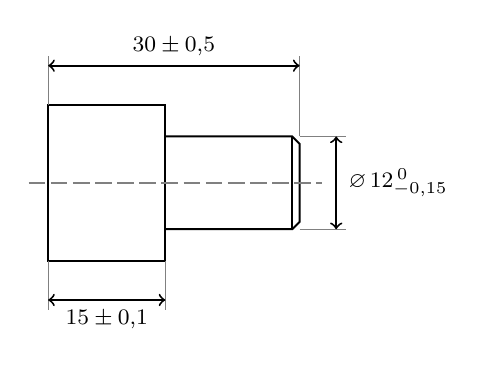
\begin{tikzpicture}[scale=0.62, line width=0.7pt, font=\footnotesize]
  \draw (0,-1.6) rectangle (2.4,1.6);
  \draw (2.4,-0.95) -- (5.0,-0.95) -- (5.15,-0.8) -- (5.15,0.8) -- (5.0,0.95) -- (2.4,0.95);
  \draw (5.0,-0.95) -- (5.0,0.95);
  \draw[dash pattern=on 6pt off 2pt, gray] (-0.4,0) -- (5.6,0);
  % cote 30 +/- 0,5
  \draw[gray, thin] (0,1.6) -- (0,2.6) (5.15,0.95) -- (5.15,2.6);
  \draw[<->] (0,2.4) -- (5.15,2.4) node[midway, above] {$30\pm 0{,}5$};
  % cote 15 +/- 0,1
  \draw[gray, thin] (0,-1.6) -- (0,-2.6) (2.4,-1.6) -- (2.4,-2.6);
  \draw[<->] (0,-2.4) -- (2.4,-2.4) node[midway, below] {$15\pm 0{,}1$};
  % cote diametre
  \draw[gray, thin] (5.15,0.95) -- (6.1,0.95) (5.15,-0.95) -- (6.1,-0.95);
  \draw[<->] (5.9,-0.95) -- (5.9,0.95);
  \node[right] at (5.95,0) {$\varnothing\,12^{\,0}_{-0{,}15}$};
\end{tikzpicture}

{\scriptsize Butée (schéma de principe, non à l'échelle)}
\end{minipage}
\end{exo}

\begin{consigne}\small
\textbf{Consignes.}
\begin{itemize}[leftmargin=12pt, itemsep=0pt, topsep=2pt]
  \item Écrire la probabilité cherchée avec la variable aléatoire \textbf{avant} tout calcul. On note $D$ le diamètre d'une pièce, en mm.
  \item Moyennes et limites au micromètre (trois décimales en mm). Écarts-types en \textmu m, à $0{,}1$ \textmu m près. Probabilités à $10^{-4}$. Dans les calculs enchaînés, \textbf{conserver les valeurs exactes}.
  \item Un réglage qui doit garantir une exigence s'arrondit \textbf{dans le sens qui respecte l'exigence}~; le dire.
  \item Calculatrice~: \texttt{normalFRép} / \texttt{Ncd} pour une probabilité, \texttt{FracNormale} / \texttt{InvN} pour un seuil (TI / Casio).
\end{itemize}
\end{consigne}

\needspace{5cm}
\begin{center}
\renewcommand{\arraystretch}{1.2}
\begin{tabular}{|>{\bfseries\centering\arraybackslash}p{1.9cm}|*{5}{>{\centering\arraybackslash}p{1.45cm}|}>{\centering\arraybackslash}p{2.2cm}|>{\centering\arraybackslash}p{2.2cm}|}
\hline
\rowcolor{uimmlightblue}
Échantillon & $M_1$ & $M_2$ & $M_3$ & $M_4$ & $M_5$ & Moyenne $\Dbar_i$ & Étendue $R_i$ \\ \hline
1 & $11{,}87$ & $11{,}86$ & $11{,}86$ & $11{,}87$ & $11{,}87$ & & \\ \hline
2 & $11{,}87$ & $11{,}87$ & $11{,}86$ & $11{,}87$ & $11{,}87$ & & \\ \hline
3 & $11{,}91$ & $11{,}90$ & $11{,}86$ & $11{,}88$ & $11{,}87$ & & \\ \hline
4 & $11{,}89$ & $11{,}90$ & $11{,}89$ & $11{,}90$ & $11{,}90$ & & \\ \hline
5 & $11{,}91$ & $11{,}90$ & $11{,}90$ & $11{,}90$ & $11{,}90$ & & \\ \hline
6 & $11{,}90$ & $11{,}91$ & $11{,}92$ & $11{,}93$ & $11{,}93$ & & \\ \hline
\end{tabular}

\smallskip
{\footnotesize Mesures du diamètre, en mm (fichier csv~: séparateur «~;~», décimale «~,~»). Colonnes à compléter en A.1.}
\end{center}

% ============================================================
\newpage
\section{Dossier de référence}

\begin{rappel}{1. Moyenne générale, étendue moyenne, écart-type du procédé}
\small
Pour $r$ échantillons de $n$ pièces, de moyennes $\Dbar_i$ et d'étendues $R_i = \max - \min$~:
\[
\Dbb = \frac{1}{r}\sum_{i=1}^{r}\Dbar_i, \qquad \Rbar = \frac{1}{r}\sum_{i=1}^{r}R_i, \qquad \sigma = \frac{\Rbar}{d_n}.
\]
Le coefficient $d_n$ est dans le tableau ci-dessous. La relation $\sigma = \Rbar/d_n$ n'a de sens que si la distribution est normale. La norme préconise de 100 à 200 relevés~; avec $30$ mesures, l'étude est préliminaire.
\end{rappel}

\begin{rappel}{2. Loi de la moyenne d'un échantillon, limites des cartes de contrôle}
\small
Si $D \sim \mathcal{N}(\mu\,;\sigma)$, la moyenne $\Dbar$ de $n$ pièces indépendantes suit $\mathcal{N}\!\left(\mu\,;\dfrac{\sigma}{\sqrt{n}}\right)$.

\smallskip
\textbf{Carte des moyennes} (procédé nouveau, $\mu$ et $\sigma$ inconnus)~:
\[
LC = \Dbb \pm A'_c\,\Rbar \quad(\text{limites de contrôle}) \qquad LS = \Dbb \pm A'_s\,\Rbar \quad(\text{limites de surveillance}).
\]
\textbf{Carte des étendues}~: $LC_2 = D'_{c2}\,\Rbar$ et $LS_2 = D'_{s2}\,\Rbar$ (limites hautes). La loi de l'étendue n'est pas normale~: on utilise le tableau.

\smallskip
Si $\mu_0$ et $\sigma_0$ sont connus~: $LC = \mu_0 \pm A_c\,\sigma_0$ et $LS = \mu_0 \pm A_s\,\sigma_0$.

\smallskip
\textbf{Convention des tables}, procédé stable~: la moyenne d'un échantillon dépasse chaque limite de contrôle avec la probabilité $0{,}001$, et chaque limite de surveillance avec la probabilité $0{,}025$.
\end{rappel}

\begin{rappel}{3. Capabilité du procédé}
\small
Avec $T_s$ et $T_i$ les bornes de la tolérance et $IT = T_s - T_i$~:
\[
C_p = \frac{IT}{6\,\sigma}, \qquad C_{pk} = \min\!\left(\frac{T_s - \mu}{3\,\sigma}\,;\ \frac{\mu - T_i}{3\,\sigma}\right) \quad\text{avec } \mu = \Dbb.
\]
$C_p$ mesure la dispersion seule. $C_{pk}$ mesure la dispersion et le centrage~: on garde la valeur minimale.

\smallskip
\begin{center}\small
\renewcommand{\arraystretch}{1.15}
\begin{tabular}{|l|l|}\hline
$C_{pk} < 1$ & le procédé n'est pas capable de maintenir toute la production dans la tolérance \\ \hline
$1 \leq C_{pk} < 1{,}33$ & minimum acceptable, il faut améliorer le procédé \\ \hline
$1{,}33 \leq C_{pk} < 2$ & indice bon \\ \hline
$C_{pk} \geq 2$ & indice excellent \\ \hline
\end{tabular}
\end{center}
\end{rappel}

\begin{rappel}{4. Coefficients pour échantillons de $n$ pièces}
\small
\begin{center}\small
\renewcommand{\arraystretch}{1.2}
\begin{tabular}{|l|*{9}{c|}}\hline
\rowcolor{white}
$n$ & 2 & 3 & 4 & 5 & 6 & 7 & 8 & 9 & 10 \\ \hline
$d_n$ & 1,128 & 1,693 & 2,059 & 2,326 & 2,534 & 2,704 & 2,847 & 2,970 & 3,078 \\ \hline
$A_c$ & 2,185 & 1,784 & 1,545 & 1,382 & 1,262 & 1,168 & 1,092 & 1,030 & 0,977 \\ \hline
$A_s$ & 1,386 & 1,132 & 0,980 & 0,876 & 0,800 & 0,741 & 0,693 & 0,653 & 0,620 \\ \hline
$A'_c$ & 1,937 & 1,054 & 0,750 & 0,594 & 0,498 & 0,432 & 0,384 & 0,347 & 0,317 \\ \hline
$A'_s$ & 1,229 & 0,668 & 0,476 & 0,377 & 0,316 & 0,274 & 0,244 & 0,220 & 0,202 \\ \hline
$D'_{c2}$ & 4,12 & 2,99 & 2,58 & 2,36 & 2,22 & 2,12 & 2,04 & 1,99 & 1,94 \\ \hline
$D'_{s2}$ & 2,81 & 2,17 & 1,93 & 1,81 & 1,72 & 1,66 & 1,62 & 1,58 & 1,56 \\ \hline
\end{tabular}
\end{center}
\end{rappel}

% ============================================================
\newpage
\section{Partie A -- Décrire le procédé \duree{[C04] [C05] -- 20 min}}

\begin{enumerate}[label={\color{uimmblue}\textbf{A.\arabic*}}, leftmargin=*]
  \needspace{6cm}
  \item\label{qA1} Compléter le tableau des mesures~: moyenne $\Dbar_i$ et étendue $R_i$ de chaque échantillon. Calculer ensuite $\Dbb$ et $\Rbar$. \tabl
  \zone{4}
  \needspace{5cm}
  \item\label{qA2} Estimer l'écart-type du procédé par $\sigma = \Rbar/d_n$. Donner $\sigma$ en \textmu m. On modélise désormais le diamètre d'une pièce par $D \sim \mathcal{N}(\mu\,;\sigma)$ avec $\mu = \Dbb$.
  \zone{3}
  \needspace{7cm}
  \item\label{qA3}
  \begin{enumerate}
    \item Donner l'intervalle $[\mu - 3\sigma\,;\mu + 3\sigma]$. Quelle proportion approximative des pièces contient-il~?
    \item Comparer cet intervalle à l'intervalle de tolérance $[11{,}85\,;12{,}00]$. Que constate-t-on~?
  \end{enumerate}
  \zone{5}
  \needspace{10.5cm}
  \item\label{qA4} \textbf{Vérifier la normalité.} Tout ce qui précède suppose que $D$ suit une loi normale. On le vérifie avec la droite de Henry.

  \begin{enumerate}
    \item Classer les $30$ mesures par ordre croissant $d_{(1)} \leq \dots \leq d_{(30)}$.
    \item Pour chaque rang $k$, calculer $p_k = \dfrac{k - 0{,}5}{30}$, puis le réel $z_k$ tel que $P(Z \leq z_k) = p_k$, où $Z \sim \mathcal{N}(0\,;1)$. C'est un problème inverse~: \texttt{FracNormale} ou \texttt{LOI.NORMALE.\allowbreak STANDARD.\allowbreak INVERSE}.
    \item Tracer les points $(d_{(k)}\,;z_k)$. Si la loi est normale, ils sont presque alignés.
    \item Conclure. Les points sont-ils bien alignés, ou voyez-vous des regroupements~? Notez ce qui vous surprend~: nous y reviendrons en partie D.
  \end{enumerate}
  \zone{4}
\end{enumerate}

% ============================================================
\needspace{9cm}
\section{Partie B -- Cartes de contrôle \duree{[C04] [C05] -- 40 min}}

\begin{enumerate}[label={\color{uimmblue}\textbf{B.\arabic*}}, leftmargin=*]
  \needspace{6cm}
  \item\label{qB1} On prélève des échantillons de $n = 5$ pièces. D'après le dossier de référence, la moyenne $\Dbar$ d'un échantillon suit $\mathcal{N}\!\left(\mu\,;\sigma/\sqrt{5}\right)$. Calculer $\sigma_{\Dbar} = \sigma/\sqrt{5}$ en \textmu m. Pourquoi les moyennes d'échantillons varient-elles moins que les pièces~?
  \zone{3}
  \needspace{11cm}
  \item\label{qB2} \textbf{Limites de la carte des moyennes.} Procédé stable, on veut $P(\Dbar > LCS) = 0{,}001$ et $P(\Dbar > LSS) = 0{,}025$, et symétriquement en bas.
  \begin{enumerate}
    \item Déterminer le réel $z_c$ tel que $P(Z > z_c) = 0{,}001$ et le réel $z_s$ tel que $P(Z > z_s) = 0{,}025$, avec $Z \sim \mathcal{N}(0\,;1)$. Attention~: la calculatrice attend l'aire \textbf{à gauche}.
    \item En déduire $LCS = \mu + z_c\,\sigma_{\Dbar}$, puis $LCI$, $LSS$ et $LSI$.
    \item Calculer $z_c/\sqrt{5}$ et $z_s/\sqrt{5}$. Les comparer aux coefficients $A_c$ et $A_s$ du tableau pour $n = 5$. Que constate-t-on~?
    \item Retrouver $LCS$ et $LSI$ avec la formule du dossier de référence ($A'_c$ et $A'_s$). Les résultats sont-ils cohérents~?
  \end{enumerate}
  \zone{8}
  \needspace{4.5cm}
  \item\label{qB3} \textbf{Limites de la carte des étendues.} Calculer $LC_2$ et $LS_2$ avec le dossier de référence.
  \zone{3}
  \needspace{5cm}
  \item\label{qB4} Tracer la carte des moyennes et la carte des étendues, avec la ligne centrale. Reporter $LCS$, $LCI$, $LC_2$ \textbf{en rouge} et $LSS$, $LSI$, $LS_2$ \textbf{en vert}. \tabl{} (grilles vierges en dernière page)
  \needspace{6cm}
  \item\label{qB5} Analyser les deux cartes~: quels points sortent des limites de contrôle~? des limites de surveillance~? Y a-t-il une tendance~? Conclure sur l'état du procédé.
  \zone{5}
  \needspace{9cm}
  \item\label{qB6} \textbf{Hasard ou cause identifiable~?}
  \begin{enumerate}
    \item Si le procédé est parfaitement stable, quelle est la probabilité qu'une moyenne d'échantillon sorte des limites de contrôle (en haut ou en bas)~?
    \item Soit $X$ le nombre de moyennes hors limites de contrôle parmi $6$ échantillons d'un procédé stable. Donner la loi de $X$, puis calculer $P(X \geq 1)$.
    \item Sur nos $6$ échantillons, $4$ moyennes sont hors limites de contrôle. L'écart-type des $6$ moyennes observées vaut $20{,}3$ \textmu m~; le comparer à $\sigma_{\Dbar}$. Conclure.
  \end{enumerate}
  \zone{6}
  \needspace{9cm}
  \item\label{qB7} \textit{Pour aller plus loin~: la carte détecte-t-elle un décalage~?} Une usure d'outil décale la moyenne du procédé de $\mu$ à $\mu + \sigma$. La moyenne d'un échantillon suit alors $\mathcal{N}(\mu + \sigma\,;\sigma_{\Dbar})$.
  \begin{enumerate}
    \item Calculer la probabilité que le prochain échantillon dépasse $LCS$. \calc
    \item Calculer la probabilité qu'au moins une alarme survienne sur les $5$ échantillons suivants.
  \end{enumerate}
  \zone{5}
\end{enumerate}

% ============================================================
\needspace{9cm}
\section{Partie C -- Capabilité du procédé \duree{[C04] [C05] -- 35 min}}

La tolérance est $T_i = 11{,}85$ et $T_s = 12{,}00$. On garde le modèle $D \sim \mathcal{N}(\mu\,;\sigma)$ des questions A.1 et A.2.

\begin{enumerate}[label={\color{uimmblue}\textbf{C.\arabic*}}, leftmargin=*]
  \needspace{6cm}
  \item\label{qC1} Calculer la proportion de pièces hors tolérance, par défaut puis par excès, en ppm ($1$ ppm $= 10^{-6}$). \calc
  \zone{4}
  \needspace{7cm}
  \item\label{qC2}
  \begin{enumerate}
    \item Calculer $C_p$ et $C_{pk}$.
    \item Conclure avec le tableau d'exploitation du dossier de référence.
    \item Pourquoi $C_p$ et $C_{pk}$ sont-ils différents~? Que vaudrait $C_{pk}$ si le procédé était centré sur le milieu de la tolérance~?
  \end{enumerate}
  \zone{6}
  \needspace{9cm}
  \item\label{qC3} \textbf{Du $C_{pk}$ aux ppm.} Pour un procédé normal, la limite la plus proche est à $z = 3\,C_{pk}$ écarts-types de la moyenne. Compléter, pour la limite la plus proche~:
  \begin{center}
  \renewcommand{\arraystretch}{1.6}
  \begin{tabular}{|>{\bfseries}p{5.2cm}|*{4}{>{\centering\arraybackslash}p{2.0cm}|}}\hline
  $C_{pk}$ & $1$ & $1{,}33$ & $1{,}67$ & $2$ \\ \hline
  $z = 3\,C_{pk}$ & & & & \\ \hline
  Pièces hors tolérance de ce côté (ppm) & & & & \\ \hline
  \end{tabular}
  \end{center}
  \smallskip
  Problème inverse~: quel $C_{pk}$ minimal garantit au plus $100$ ppm de pièces hors tolérance du côté critique~? Arrondir au centième dans le sens qui respecte l'exigence. \calc
  \zone{3}
  \needspace{9cm}
  \item\label{qC4} \textbf{Fenêtre de réglage.} On garde $\sigma$. On exige au plus $100$ ppm de pièces hors tolérance \textbf{de chaque côté}.
  \begin{enumerate}
    \item Déterminer la valeur minimale de $\mu$, au micromètre, dans le sens qui respecte l'exigence.
    \item Déterminer la valeur maximale de $\mu$, dans les mêmes conditions.
    \item Où se situe le réglage actuel $\mu = \Dbb$ dans cette fenêtre~? Quelle est sa marge de sécurité~?
  \end{enumerate}
  \zone{7}
  \needspace{7cm}
  \item\label{qC5} \textbf{Dispersion maximale.} Le client veut au plus $50$ ppm de pièces hors tolérance \emph{au total}, avec un procédé centré sur $11{,}925$. Déterminer l'écart-type maximal $\sigma_{\max}$, en \textmu m, arrondi à $0{,}1$ \textmu m dans le sens qui respecte l'exigence. Le comparer à $\sigma$.
  \zone{5}
\end{enumerate}

% ============================================================
\needspace{9cm}
\section{Partie D -- Synthèse et décision \duree{[C04] [C05] -- 15 min}}

\begin{enumerate}[label={\color{uimmblue}\textbf{D.\arabic*}}, leftmargin=*]
  \needspace{7cm}
  \item\label{qD1} \textbf{Sur la durée.} Prendre maintenant les $30$ mesures \emph{ensemble}.
  \begin{enumerate}
    \item Calculer leur écart-type $s$, en \textmu m. Le comparer à $\sigma = \Rbar/d_n$.
    \item Recalculer $C_p$ et $C_{pk}$ avec $s$ à la place de $\sigma$. Que devient la conclusion~?
    \item Expliquer l'écart entre $s$ et $\sigma$ avec ce que vous avez vu sur les cartes et sur la droite de Henry.
  \end{enumerate}
  \zone{7}
  \needspace{6cm}
  \item\label{qD2} \textbf{Photographie échantillon par échantillon.} On garde $\sigma$ et on prend pour $\mu$ la moyenne de l'échantillon~: calculer la proportion de pièces en dessous de $T_i$ pour l'échantillon $1$, puis pour l'échantillon $6$. Qu'en déduire sur le $C_{pk}$ global de la question C.2~? \calc
  \zone{4}
  \needspace{7cm}
  \item\label{qD3} \textbf{Décision.} La moyenne des échantillons évolue d'environ $10$ \textmu m par échantillon. Si cette dérive se poursuit au même rythme, au bout de combien d'échantillons la moyenne atteint-elle la borne haute de la fenêtre de la question C.4~? Proposer deux actions pour le régleur et le technicien méthodes.
  \zone{6}
\end{enumerate}

% ============================================================
\newpage
\section{Dossier réponse -- cartes de contrôle}

\noindent\textbf{Carte de contrôle de la moyenne} \quad $\Dbar_i$ (mm)
\medskip

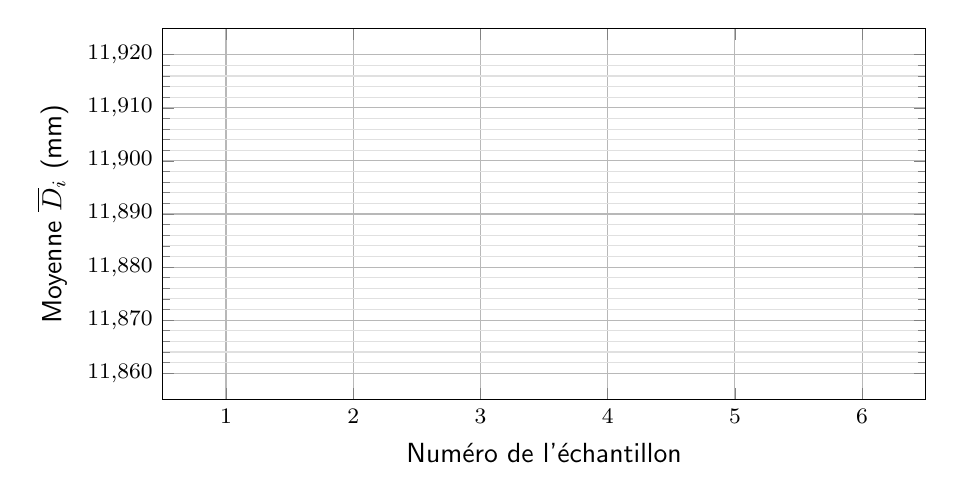
\begin{tikzpicture}
\begin{axis}[ctl, ymin=11.855, ymax=11.925, ytick={11.86,11.87,11.88,11.89,11.90,11.91,11.92}, ylabel={Moyenne $\Dbar_i$ (mm)}]
\end{axis}
\end{tikzpicture}

\bigskip
\noindent\textbf{Carte de contrôle de l'étendue} \quad $R_i$ (mm)
\medskip

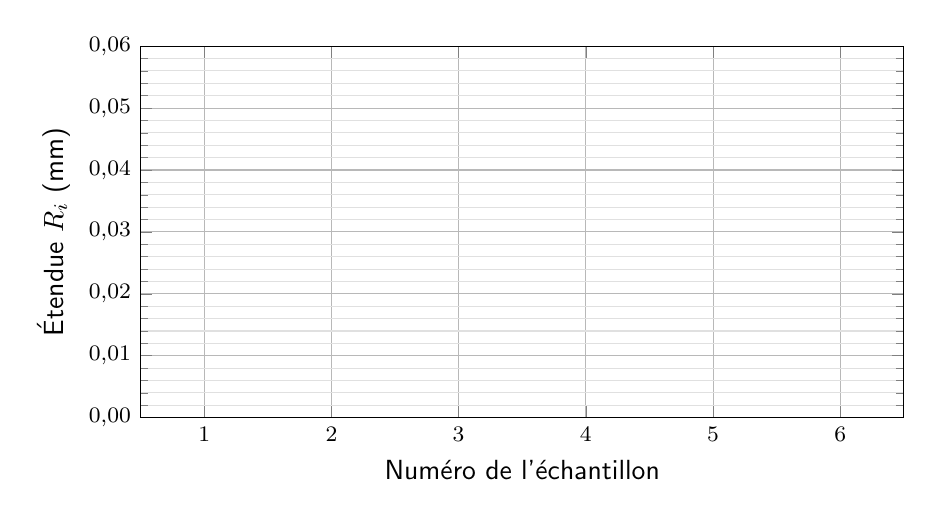
\begin{tikzpicture}
\begin{axis}[ctl, ymin=0, ymax=0.06, ytick={0,0.01,0.02,0.03,0.04,0.05,0.06}, ylabel={Étendue $R_i$ (mm)}, yticklabel style={/pgf/number format/precision=2}]
\end{axis}
\end{tikzpicture}

\end{document}
